% Header: Here are all packages used and some additional definitions
%%%%%%%%%%%%%%%%%%%%%%%%%%%%%%%%%%%%%%%%%%%%%%%%%%%%%%%%%%%%%%%%%%%

\documentclass[11pt,a4paper]{scrartcl}
\usepackage[margin=2.5cm]{geometry}
\usepackage[onehalfspacing]{setspace}
\usepackage{graphicx} % zum Einbinden von Graphiken
\usepackage[breaklinks=true,colorlinks=true,linkcolor=blue,urlcolor=blue,citecolor=blue]{hyperref} % f. Referenzen
\usepackage{amsmath,amsthm,amssymb} % Mathematik Umgebung 
\usepackage{icomma} % Intelligentes Komma, das den richtigen Abstand zwischen Dezimalzahlen als auch in Formeln wählt.
\usepackage[ngerman]{babel} % Deutsche Bezeichnungen bei Inhaltsangabe etc
\usepackage[T1]{fontenc}    % andere Schriftsatzkodierung für richtige Silbentrennung bei Umlauten
\usepackage[locale = DE,space-before-unit=true,per-mode = symbol]{siunitx} % Bessere Einheiten
\usepackage{booktabs,multirow} % Pakete zur Erstellung von Tabellen
\usepackage{placeins} % Definiert den Befehl “\FloatBarrier”, der die Ausgabe der davor eingebundenen Bilder erzwingt, befor der Text weiter geht. (Mit vorsicht zu verwenden)
\usepackage[natbib,abbreviate=true,doi=false,style=numeric-comp,giveninits=true,sorting=none]{biblatex} % Modernes Paket zur Erzeugung von Bibliografien (benötigt biber!)
\usepackage{csquotes} % Fortgeschrittene Funktionen für Zitate, für die deutsche Form der Anführungszeichen bei Referenzen
\usepackage{fancyhdr}
\usepackage{enumitem}
\usepackage{float} 
\usepackage{graphicx}
\addbibresource{MyBibliography.bib} % Ort der .bib Datei, die die Datenbank für Literatur/ Referenzen enthält.

% Redefine names for figures, tables, and contents
\addto\captionsngerman{
  \renewcommand{\figureautorefname}{Abbildung} 
  \renewcommand{\sectionautorefname}{Kapitel} 
  \renewcommand{\subsectionautorefname}{Unterkapitel} 
}
\selectlanguage{ngerman}


\graphicspath{{Bilder/}}

\DeclareSIUnit{\dBm}{dBm}
\DeclareSIUnit[per-mode=reciprocal]\WN{\per\centi\meter}

%header:
\pagestyle{fancy}
\fancyhf{}
\fancyhfoffset[L]{1cm} % left extra length
\fancyhfoffset[R]{1cm} % right extra length
\rhead{\today}
\lhead{Numerische Integration und Normalverteilung}
\fancyfoot[C]{\thepage}
%%%%%%%%%%%%%%%%%%%%%%%%%%%%%%%%%%%%%%%%%%%%%%%%%%%%%%%%%%%%%%%%%%%
\begin{document}
%
\titlehead{
\includegraphics[width=5cm]{dhbw.pdf}}
\title{Numerische Integration und Normalverteilung}
\author{Carl-Ferdinand Oliver\thanks{\href{mailto:es23035@lehre.dhbw-stuttgart.de}{es23035@lehre.dhbw-stuttgart.de}}, Tom Springer \thanks{\href{mailto:es23026@lehre.dhbw-stuttgart.de}{es23026@lehre.dhbw-stuttgart.de}}, Jonas Münz \thanks{\href{mailto:es23039@lehre.dhbw-stuttgart.de}{es23039@lehre.dhbw-stuttgart.de}}, \\ Max Valentin Orlemann \thanks{\href{mailto:es23023@lehre.dhbw-stuttgart.de}{es23023@lehre.dhbw-stuttgart.de}}, Alexander Kögel \thanks{\href{mailto:es23031@lehre.dhbw-stuttgart.de}{es23031@lehre.dhbw-stuttgart.de}}\\TES23}
\date{\today}
\maketitle
\vfill

\thispagestyle{empty}
%
%
\tableofcontents
\thispagestyle{empty}
\cleardoublepage
\pagenumbering{arabic} 
\newpage
%
%

%%%%%%%%%%%%%%%%%%%%%%%%%%%%%%%%%%%%%%%%
%Statistische Grundlagen
\section{Statistische Grundlagen}
\label{sec:statistische_grundlagen}

\subsection{Normalverteilung}
\label{sec:normal_distribution}
Die Gaußsche Normalverteilung beschreibt die Verteilung einer stetigen Zufallsvariablen und ist durch zwei Parameter, den Mittelwert $\mu$ und die Standardabweichung $\sigma$, charakterisiert. Sie wird auch als \textit{Glockenkurve} bezeichnet und ist symmetrisch um den Mittelwert.

\subsection*{Wichtige Eigenschaften}
\begin{itemize}
    \item Die Dichtefunktion der Normalverteilung lautet:
    \[
    f(x) = \frac{1}{\sqrt{2 \pi} \sigma} \cdot \exp\left(-\frac{(x - \mu)^2}{2 \sigma^2}\right)
    \]
    \item Die Verteilungsfunktion ist gegeben durch:
    \[
    \Phi(x) = P(X \leq x) = \int_{-\infty}^{x} f(t) \, dt
    \]
    \item Die Normalverteilung ist symmetrisch zum Mittelwert $\mu$, hat ein Maximum bei $x = \mu$ und Wendepunkte bei $x = \mu \pm \sigma$.
    \item Sie ist normiert, d.h., das Integral über die gesamte Dichtefunktion ergibt 1:
    \[
    \int_{-\infty}^{\infty} f(x) \, dx = 1
    \]
\end{itemize}

\subsection*{Berechnung der Wahrscheinlichkeiten}
Für die Berechnung von Wahrscheinlichkeiten, die der Gaußschen Normalverteilung folgen, werden in der Praxis oft Tabellen oder numerische Verfahren verwendet, da die Integrale analytisch nicht lösbar sind. Die Wahrscheinlichkeit für einen Bereich $a \leq X \leq b$ kann mit der Verteilungsfunktion berechnet werden:
\[
P(a \leq X \leq b) = \Phi\left(\frac{b - \mu}{\sigma}\right) - \Phi\left(\frac{a - \mu}{\sigma}\right)
\]

\subsection*{Wahrscheinlichkeiten in Abhängigkeit der Standardabweichung}

Da die Normalverteilung symmetrisch um den Mittelwert $\mu$ ist, lassen sich bestimmte Wahrscheinlichkeitsbereiche in Abhängigkeit von der Standardabweichung $\sigma$ um $\mu$ angeben:

\begin{itemize}
    \item Etwa 68,27\% aller Werte einer normalverteilten Zufallsvariablen liegen im Intervall $[\mu - \sigma, \mu + \sigma]$, also innerhalb einer Standardabweichung um den Mittelwert.
    \item Etwa 95,45\% der Werte befinden sich im Intervall $[\mu - 2\sigma, \mu + 2\sigma]$, also innerhalb von zwei Standardabweichungen.
    \item Rund 99,73\% der Werte liegen im Intervall $[\mu - 3\sigma, \mu + 3\sigma]$, also innerhalb von drei Standardabweichungen.
\end{itemize}
Diese Bereiche werden auch als \textit{Empirische Regel} oder \textit{68-95-99,7-Regel} bezeichnet und sind besonders nützlich zur Einschätzung, wie wahrscheinlich es ist, dass eine Zufallsvariable in einem bestimmten Bereich um den Mittelwert liegt. Die Wahrscheinlichkeit, dass ein Wert weiter als $3\sigma$ vom Mittelwert entfernt liegt, ist sehr gering und beträgt nur ca. 0,27\%. \\
In der Praxis wird die Normalverteilung zur Modellierung vieler realer Phänomene verwendet, wie z.B. Fehlerverteilungen, Körpergrößen oder IQ-Werte, da viele natürliche
Prozesse einem normalverteilten Muster folgen. \cite{skript_statistik}


\subsection{Standardnormalverteilung}
\label{sec:standard_normal_distribution}

Eine Normalverteilung lässt sich durch die Standardisierung mit $z = \frac{x - \mu}{\sigma}$ auf die sogenannte Standardnormalverteilung $\mathcal{N}(0, 1)$ zurückführen, die Mittelwert 0 und Standardabweichung 1 hat:
\[
\phi(z) = \frac{1}{\sqrt{2 \pi}} \cdot \exp\left(-\frac{z^2}{2}\right)
\]
Die Standardnormalverteilung ist ein nützliches Werkzeug in der Statistik, da sie es ermöglicht, beliebige Normalverteilungen durch eine Transformation auf diese Standardform zu bringen. Dies wird durch die Berechnung des \textit{z-Scores} erreicht:
\[
z = \frac{X - \mu}{\sigma}
\]
Der z-Wert gibt an, wie viele Standardabweichungen ein Wert \(X\) vom Mittelwert entfernt ist. Diese Transformation erleichtert die Berechnung von Wahrscheinlichkeiten und statistischen Tests, da die Eigenschaften der Standardnormalverteilung bekannt sind und in Tabellen dokumentiert werden.


\subsection{t-Student-Verteilung}
\label{sec:t_student_distribution}
Die standardisierte Schätzfunktion des Stichprobenmittelwerts normalverteilter Daten ist nicht mehr normalverteilt, sondern \(t\)-verteilt, wenn die zur Standardisierung des Mittelwerts benötigte Varianz des Merkmals unbekannt ist und mit der Stichprobenvarianz geschätzt werden muss. Seine \(t\)-Verteilung ermöglicht die Berechnung der Verteilung der Differenz zwischen dem Mittelwert der Stichprobe und dem wahren Mittelwert der Grundgesamtheit. \\
Die \(t\)-Werte hängen vom Signifikanzniveau sowie von der Stichprobengröße \(n\) ab und bestimmen das Vertrauensintervall sowie die Aussagekraft der Schätzung des Mittelwertes. Die \(t\)-Verteilung wird mit wachsendem \(n\) schmaler und konvergiert für \(n \to \infty\) zur Standardnormalverteilung. Hypothesentests, bei denen die \(t\)-Verteilung Verwendung findet, bezeichnet man als \(t\)-Tests. \cite{studenten_t_verteilung}\\
Die t-Student-Verteilung wird verwendet, wenn die Stichprobengröße klein ist (\(n < 30\)) und die Varianz der Grundgesamtheit unbekannt ist. Sie ähnelt der Normalverteilung, hat jedoch „schwerere“ Ränder. Dies bedeutet, dass extremere Werte wahrscheinlicher sind als bei der Normalverteilung.
Die t-Student-Verteilung hat einen Parameter, die Freiheitsgrade \(df\), der die Form der Verteilung bestimmt. Je größer die Freiheitsgrade, desto mehr nähert sich die t-Verteilung der Normalverteilung an. Bei einer großen Stichprobengröße (ca. \(df > 30\)) ist der Unterschied zur Normalverteilung vernachlässigbar.
In der Statistik wird die t-Verteilung häufig für Hypothesentests verwendet. Sie spielt auch bei der Berechnung von Konfidenzintervallen eine wichtige Rolle, wenn die Varianz der Grundgesamtheit nicht bekannt ist.


\subsection{$\chi^2$-Verteilung}
\label{sec:chi_square_distribution}
\begin{figure}[h]
    \centering
    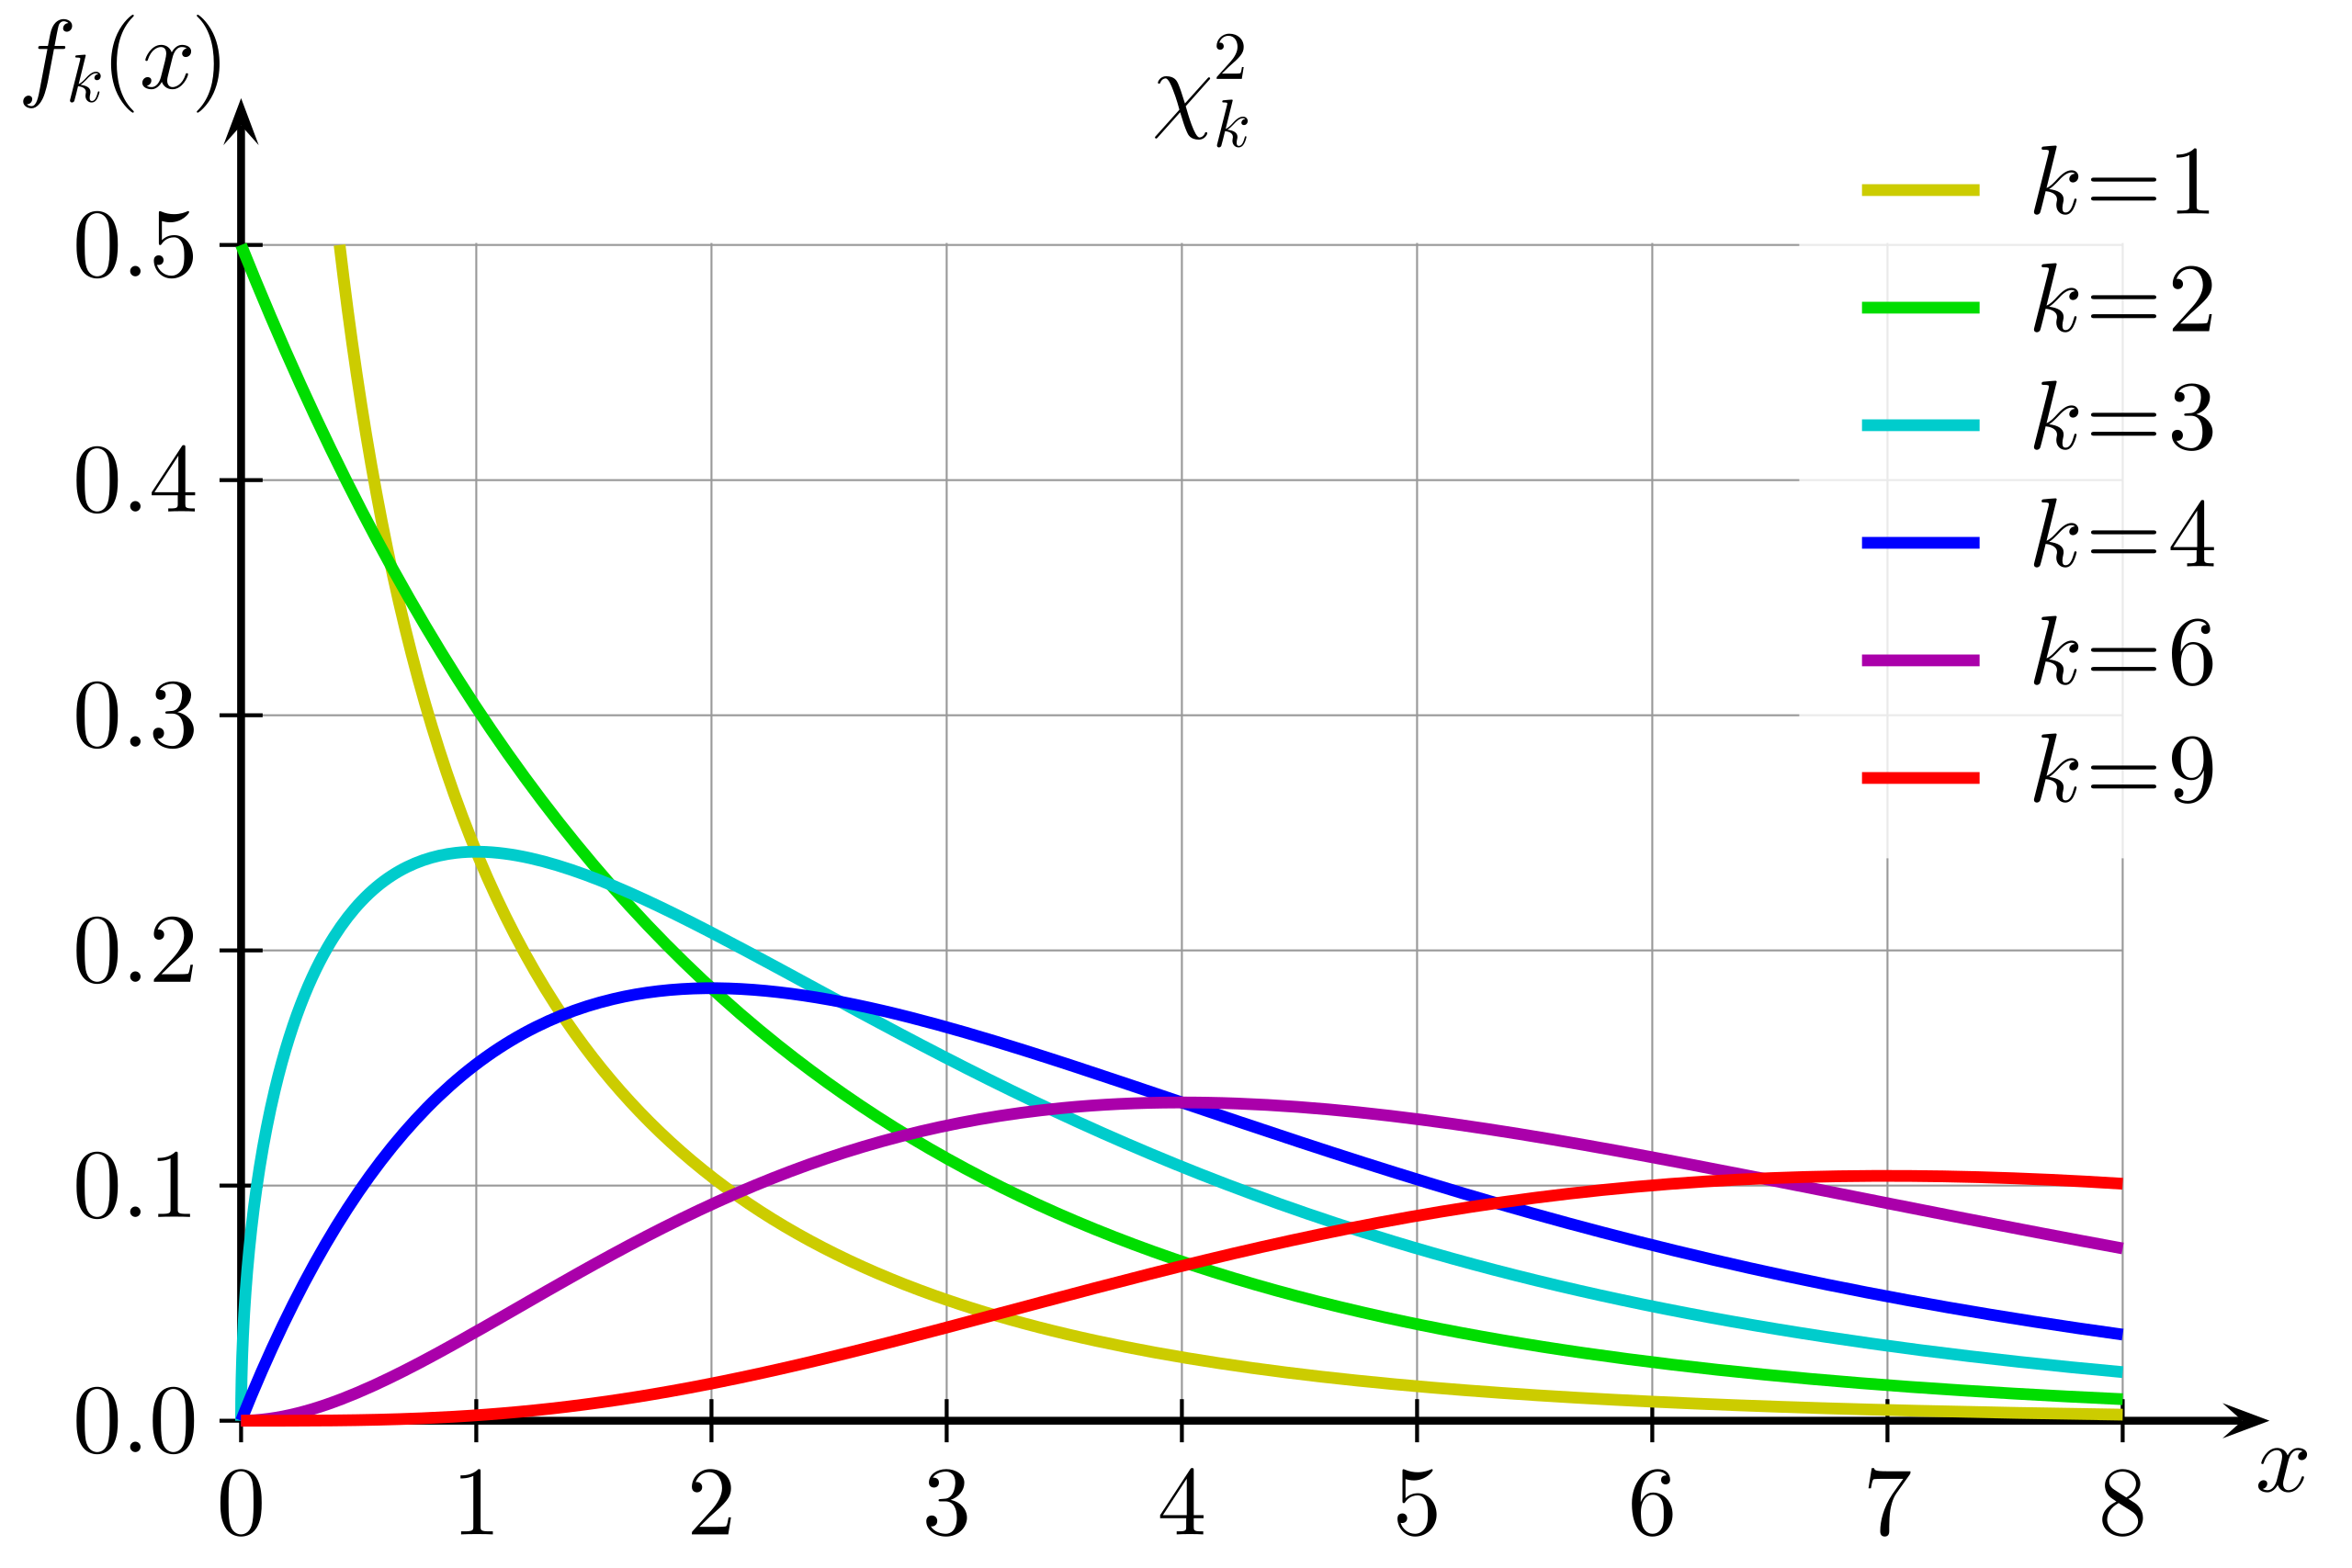
\includegraphics[width=8cm]{Bilder/chi^2-distribution.png}
    \caption{
        Weitere Einzelheiten
        Dichten der Chi-Quadrat-Verteilung mit unterschiedlicher Anzahl an Freiheitsgraden k \cite{chi^2_distribution}}    
    \label{fig:keplersche_fassregel}
\end{figure}
Die \textbf{$\chi^2$-Verteilung} entsteht als Summe der quadrierten z-Werte aus einer Standardnormalverteilung. Sie wird häufig in der Statistik verwendet, um Varianzen zu schätzen und in Hypothesentests wie dem \textit{Chi²-Anpassungstest} oder dem \textit{Chi²-Test zur Unabhängigkeit}.
Die Chi²-Verteilung hat einen Parameter, die Freiheitsgrade \(df\), der die Form der Verteilung bestimmt. Sie ist asymmetrisch und nur für positive Werte definiert. Für \(df \geq 30\) nähert sich die Chi²-Verteilung zunehmend der Normalverteilung an.
Ein häufiges Anwendungsgebiet der Chi²-Verteilung ist die Analyse von Kontingenztafeln, bei denen überprüft wird, ob zwei kategorische Variablen unabhängig voneinander sind.



%%%%%%%%%%%%%%%%%%%%%%%%%%%%%%%%%%%%%%%%
%Statistische Grundlagen

\section{Trapezregel}
\label{sec:trapezregel}

\subsection{Herleitung}
\label{sec:herleitung}

\begin{figure}[h]
    \centering
    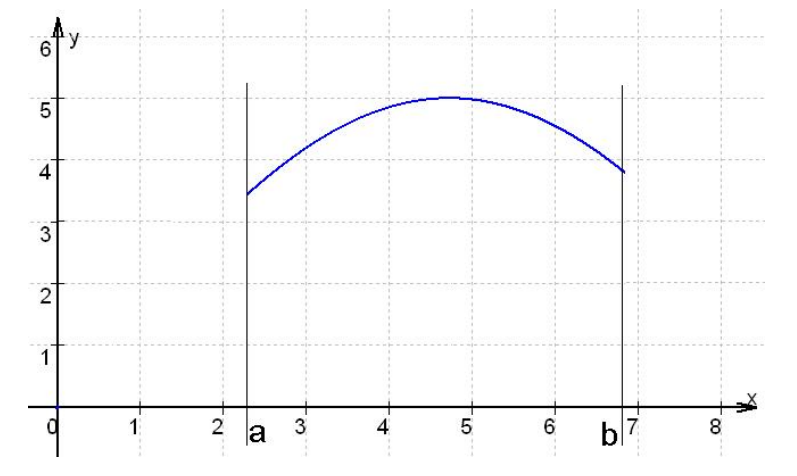
\includegraphics[width=8cm]{Bilder/keplersche_fassregel_funktion.png}
    \caption{Keplersche Fassregel \cite{skript}}    
    \label{fig:keplersche_fassregel}
    \end{figure}

\subsection{Fehlerabschätzung}
\label{sec:fehlerabschätzung}

\subsection{Vertrauensniveau $\gamma$}
\label{sec:vertrauensniveau}

\subsection{Alternativen zur Trapezregel} 
\label{sec:alternativen}


%%%%%%%%%%%%%%%%%%%%%%%%%%%%%%%%%%%%%%%%

%Statistische Grundlagen

\section{Umsetzung im Programm}
\label{sec:umsetzung_im_programm}

\subsection{Berechnung des Mittelwerts}
Der Mittelwert (\(\mu\)) der Daten wird berechnet, indem die Summe aller Datenpunkte durch die Anzahl der Punkte (\(n\)) geteilt wird:
\[
\mu = \frac{1}{n} \sum_{i=1}^{n} A_i
\]

\subsection{Berechnung der Varianz}
Die Varianz (\(\sigma^2\)) wird berechnet, um zu messen, wie die Daten um den Mittelwert streuen. Der Code verwendet die Formel für die erwartungstreue Varianz:
\[
\sigma^2 = \frac{1}{n-1} \sum_{i=1}^{n} (A_i - \mu)^2
\]
Die Verwendung von \(n-1\) anstelle von \(n\) ist wichtig, um eine Verzerrung der Schätzung zu vermeiden (Bessel-Korrektur).

\subsection{Berechnung der Konstante \(c\) durch numerische Integration}
Der Code verwendet die Trapezregel, um die Fläche unter der Standardnormalverteilung zu berechnen. Die Trapezregel ist eine numerische Methode zur Approximation des Integrals einer Funktion.

\subsubsection{Ziel der Berechnung}
Die Fläche unter der Standardnormalverteilung wird so lange berechnet, bis sie einen bestimmten Zielwert erreicht, der durch \((\gamma + 1) / 2\) definiert ist. Dies entspricht dem gewünschten Konfidenzniveau (z. B. 99\% oder 0,99).

\subsubsection{Funktion der Standardnormalverteilung}
Die Funktion \texttt{standardnormalverteilung(x)} berechnet den Wert der Standardnormalverteilung für einen gegebenen Wert \(x\):
\[
f(x) = \frac{1}{\sqrt{2\pi}} e^{-\frac{x^2}{2}}
\]

\subsection{Berechnung des Konfidenzintervalls}
Nach der Berechnung der Konstante \(c\) wird das Konfidenzintervall mit der folgenden Formel berechnet:
\[
\text{Oben} = \mu + c \cdot \sqrt{\frac{\sigma^2}{n}}
\]
\[
\text{Unten} = \mu - c \cdot \sqrt{\frac{\sigma^2}{n}}
\]
Dies gibt das Konfidenzintervall an, in dem mit einer bestimmten Wahrscheinlichkeit (z.B. 99\%) der wahre Mittelwert der Grundgesamtheit liegt.


%
\printbibliography[]
\vfill


\end{document}
